\documentclass[a4paper]{report}
\usepackage[italian]{babel}
\usepackage[utf8]{inputenc}
\usepackage{hyperref, graphicx, colortbl, gensymb}

\title{Calore}
\author{Federico Boz}
\date{Giugno 2019}

\begin{document}

\maketitle
\tableofcontents

\chapter*{Introduzione}
    In termodinamica e in termochimica, il calore è definito come il contributo di energia trasformata a seguito di una reazione chimica o nucleare e trasferita tra due sistemi o tra due parti dello stesso sistema, non imputabile ad un lavoro o ad una conversione tra due differenti tipi di energia. Il calore quindi è una forma di energia trasferita e non una forma di energia contenuta come l'energia interna.
    \newline
    Durante la prima metà del Settecento gli studiosi ricorrevano alla sostanza elementare denominata flogisto per spiegare il riscaldamento di alcuni materiali e la combustione.
    Negli anni successivi i fenomeni termici vennero ricondotti alla teoria secondo la quale il calore era un fluido non visibile, che entrando dentro la materia di un corpo poteva aumentarne la temperatura.
    Nonostante gli studi seicenteschi di Boyle sulla relazione tra il moto delle particelle e il calore, solamente verso metà del XIX secolo si gettarono le basi della termodinamica, grazie agli studi di Mayer (1842) e Joule (1843), riguardanti la quantità di calore e il lavoro necessario per ottenerlo.
    
\chapter{Calore in ambito scientifico}
\section{Unità di misura}
    In quanto energia scambiata, il calore si misura nel Sistema Internazionale in joule. Nella pratica viene tuttavia ancora spesso usata come unità di misura la caloria, che è definita come la quantità di calore necessaria a portare la temperatura di un grammo di acqua distillata, sottoposta alla pressione di 1 atm, da 14,5 \degree C a 15,5 \degree C. A volte si utilizzano anche unità a carattere meramente tecnico, quali kWh o BTU.
    
    
    Alcune equivalenze:
    \newline
    \begin{table}[htbp]
        \centering
            \begin{tabular}{|c|c|c|c|c|c|}
                \hline
                & KJ & kWh & kcal & BTU & $kg_p*m$ \\\hline
                1 kJ & 1 &	$2,778*10^{-4}$ &	0,2388 &	0,9478 &	$1,020*10^{-2}$\\ \hline
                1 kWh &	3600 &	1 &	859,8 &	3412 &	$3,671*10^5$ \\ \hline
                1 kcal & 4,187 & $1,163*10^{-3}$ &	1 & 3,968 &	$4,269*10^2$ \\ \hline
                1 BTU & 1,055 & $2,941*10^{-4}$ & 0,2519 & 1 & $1,076*10^{-2}$ \\ \hline
                1 $kg_p*m$ & $9,807*10^{-3}$ & $2,721*10^{-6}$ & $2,342*10{-3}$ &	$9,295*10^{-3}$ & 1 \\ \hline
            \end{tabular}
    \end{table}

\section{Passaggio di calore}
    Gli effetti del passaggio di calore sono descritti dal primo principio della termodinamica nella sua forma più generale:
    
    $\Delta E=Q-W$

    dove $\Delta E$ indica una variazione di qualsiasi forma di energia (ad esempio energia interna, cinetica, potenziale), Q indica il calore e W indica il lavoro (per variazione di volume o isocoro). Le conseguenze del passaggio di calore possono quindi essere principalmente di due tipi: variazione di energia o scambio di lavoro.

    Una particolare forma di energia che può essere modificata a seguito del passaggio di calore è l'energia interna; la variazione di energia interna può avere diverse conseguenze, tra cui una variazione di temperatura o un cambiamento di stato di aggregazione.

    Se il trasferimento di calore ha come conseguenza un cambiamento di stato di aggregazione, tale calore prende il nome di calore latente, mentre se il trasferimento di calore ha come conseguenza una diminuzione della differenza di temperatura (in quanto i due sistemi o le due parti dello stesso sistema tendono a raggiungere l'equilibrio termico) si parla di calore sensibile.

    La classica formula del calore sensibile è:
    
    $Q=c*m*{\Delta T}$
    
    mentre quelal del calore latente è:
    
    $Q=\lambda * m$
    
    Infine nel caso in cui il trasferimento di calore comporti sia una diminuzione della differenza di temperatura sia un cambiamento di fase, tale calore può essere pensato come la somma di due contributi: un contributo relativo al calore sensibile e un contributo relativo al calore latente.

    Ad esempio l'aumento di temperatura dell'acqua da 20 $\degree$ C a 50 $\degree$ C in condizioni standard (cioè alla pressione di 1 atm) è determinato dal fatto che ad essa è fornito calore sensibile, mentre, se l'acqua ha già raggiunto la temperatura d'ebollizione, essa immagazzina energia (sotto forma di calore latente), mantenendo la propria temperatura invariata, fino a quando non avviene il cambiamento di fase da liquido a vapore. Per tale motivo, un getto di vapore acqueo a 100 $\degree$ C, avendo immagazzinato energia durante il passaggio di stato, può provocare ustioni più gravi dell'acqua allo stato liquido alla medesima temperatura.

    Si parla inoltre di "calore di reazione" quando il calore viene consumato o generato da una reazione chimica.

\subsection{Propagazione del calore}
    Il trasferimento (o scambio o propagazione) del calore tra sistemi può avvenire in tre modi:
    
    \begin{itemize}
        \item per conduzione: in uno stesso corpo o fra corpi a contatto si ha una trasmissione, per urti, di energia cinetica tra le molecole appartenenti a zone limitrofe del materiale. Nella conduzione viene trasferita energia attraverso la materia, ma senza movimento macroscopico di quest'ultima;
        
        \item per convezione: in un fluido in movimento, porzioni del fluido possono scaldarsi o raffreddarsi per conduzione venendo a contatto con superfici esterne e poi, nel corso del loro moto (spesso a carattere turbolento), trasferire (sempre per conduzione) l'energia acquistata ad altre superfici, dando così luogo ad un trasferimento di calore per avvezione. In un campo gravitazionale quale quello terrestre (associato alla forza peso), tale modalità di trasferimento di calore, detta convezione libera, è dovuta al naturale prodursi di correnti avvettive, calde verso l'alto e fredde verso il basso, dovute a diversità di temperatura e quindi di densità delle regioni di fluido coinvolte nel fenomeno, rispetto a quelle del fluido circostante;
        
        \item per irraggiamento: tra due sistemi la trasmissione di calore può avvenire a distanza (anche nel vuoto), per emissione, propagazione e assorbimento di onde elettromagnetiche: anche in questo caso il corpo a temperatura inferiore si riscalda e quello a temperatura superiore si raffredda.[4] Il meccanismo dell'irraggiamento non richiede il contatto fisico tra i corpi coinvolti nel processo.
    \end{itemize}
    
    \begin{figure}
        \centering
        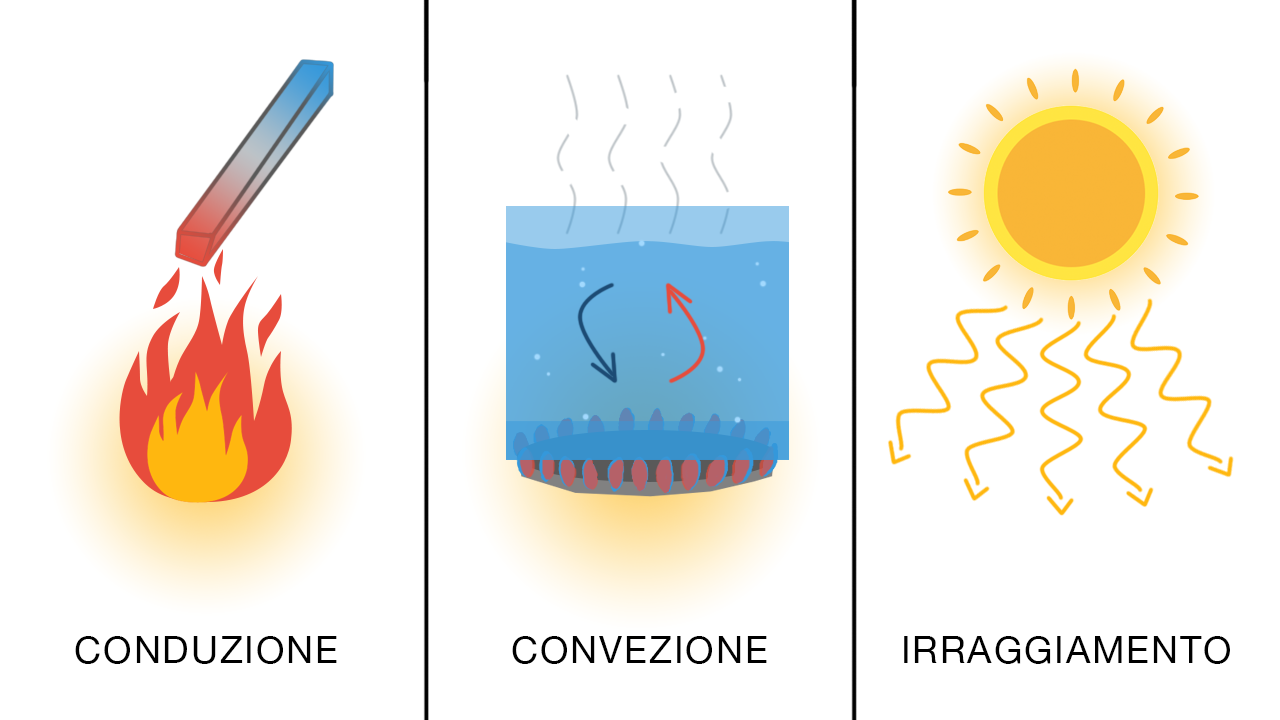
\includegraphics[scale=0.4]{calore}
        \caption{Propagazione del calore}
    \end{figure}
    
    
Nella pratica tecnica e nell'impiantistica in genere lo scambio di calore senza mescolamento tra fluidi diversi avviene in dispositivi appositamente progettati, chiamati appunto scambiatori di calore.

      \begin{figure}
        \centering
        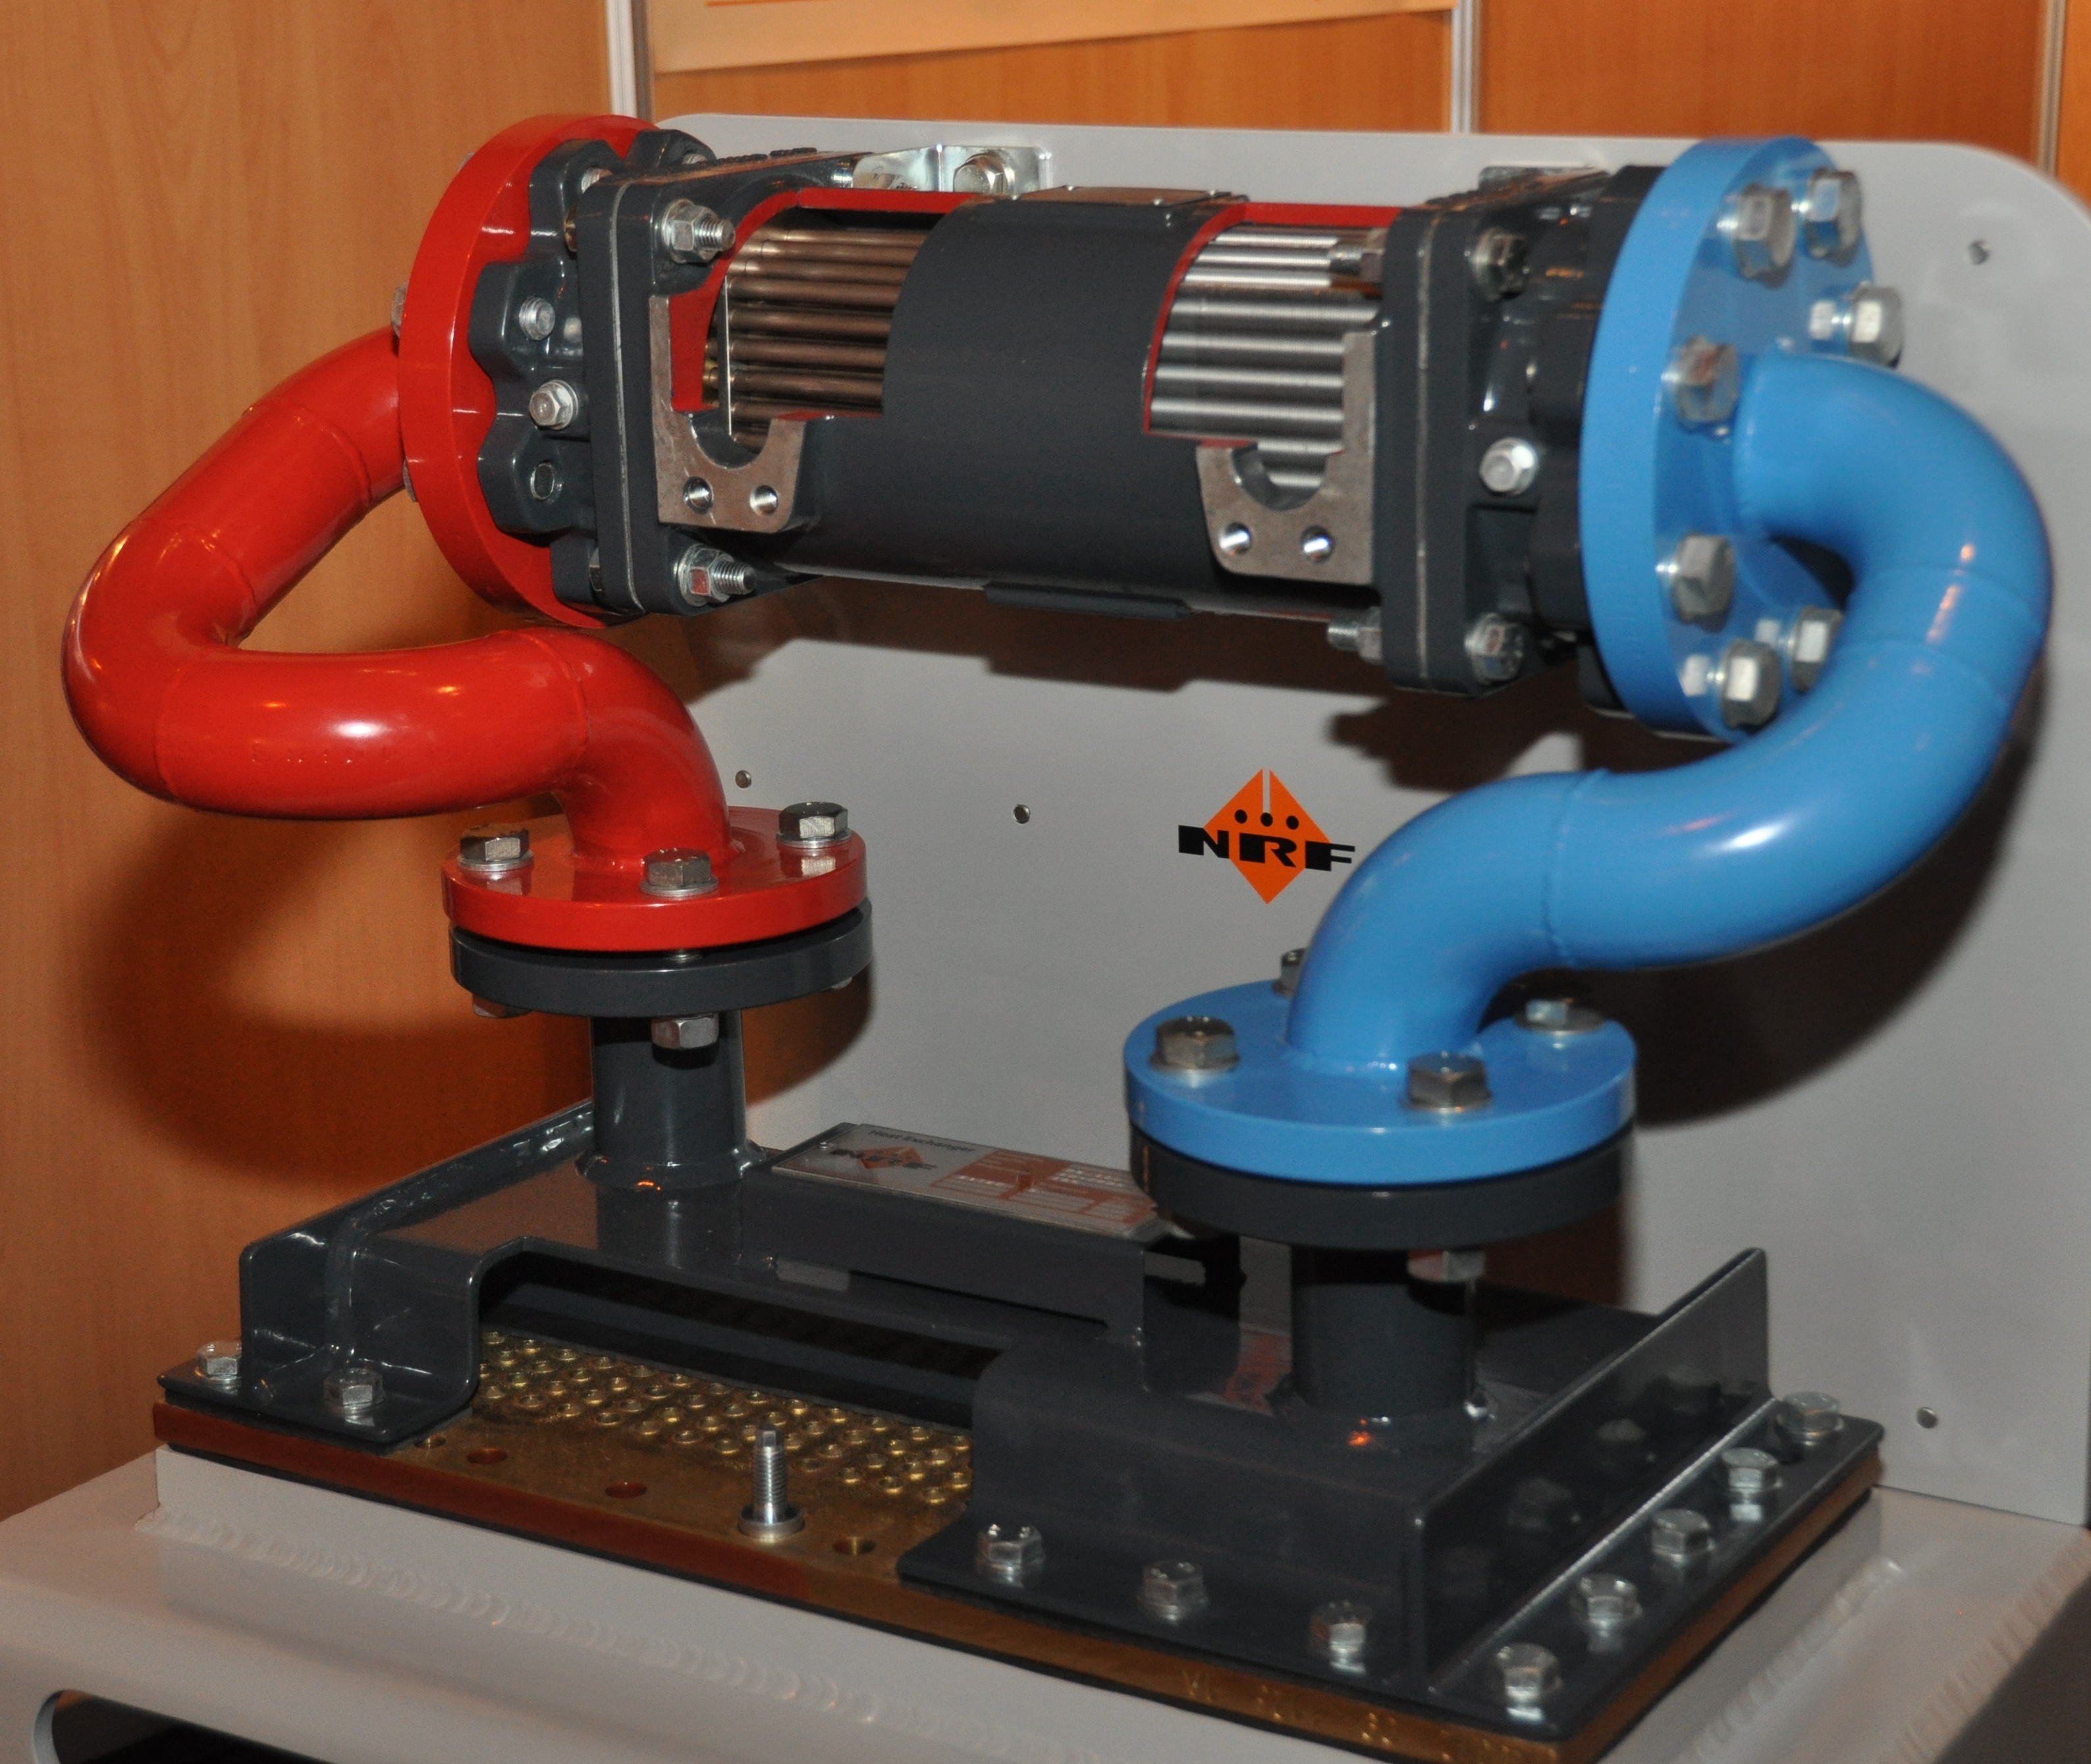
\includegraphics[scale=0.2]{heat}
        \caption{Scambiatore di calore}
    \end{figure}

\end{document}
